
\documentclass{article}
\usepackage{graphicx}
\graphicspath{{images/}}
\usepackage{hyperref}
\usepackage{listings}
\usepackage[usenames,dvipsnames,svgnames,table]{xcolor}
\usepackage{titlesec}
\usepackage{color}

\title{TP 4A - Génie Logiciel
Programme Java intégrant modélisation UML, versionning (git)
et tests unitaires (Junit)
}



\author{Mathis Vaugeois - Tanguy Moriceau -  Faustine Guillou}

\date{January 2023}

\begin{document}

\maketitle
\tableofcontents

\newpage
\section{Introduction}
\newline
\subsection{Contexte}
Ce TP final nous a permis de mettre en pratique tout ce que nous avions pu étudier et apprendre pendant les cours de Génie Logiciel.
Nous avons créé une application de gestion d'un dossier bancaire. En premier lieu, pour bien organiser notre projet, nous avons commencé par réaliser des diagrammes. Nous avons mis en pratique ce que nous avions appris de la gestion des versions, pour travailler en équipe. De plus, nous avons utilisé les tests unitaires pour vérifier notre code.

\subsection{Git}
Pour faciliter les échanges de fichiers au sein du groupe, nous avons décidé d'utiliser github et plus particulièrement sont interfaces github desktop. Cela permet de facilement voir les changements des "commits" avant de les "push", l'historique, de changer de branche, ... Pour faire ceci, nous avons d'abord créé un projet sur github, qu'on s'est partagé pour pouvoir modifier directement dessus et non sur un clone. Nous avons ensuite créé différentes branches car travailler à plusieurs sur la même peut produire des conflits avec les différentes versions que l'on a push (ou pull) et donc séparer l'espace de travail permet de sauvegarder et récupérer la version à jour de la main avant de merge avec celle-ci pour limiter les bugs. Nous avons donc effectué de nombreux commit et push durant ce TP et pour mieux nous y retrouver, nous avons commenté certains commit avec un titre et une description facilitant la lecture et la compréhension des changements produits par le groupe. 
\begin{figure}[h]
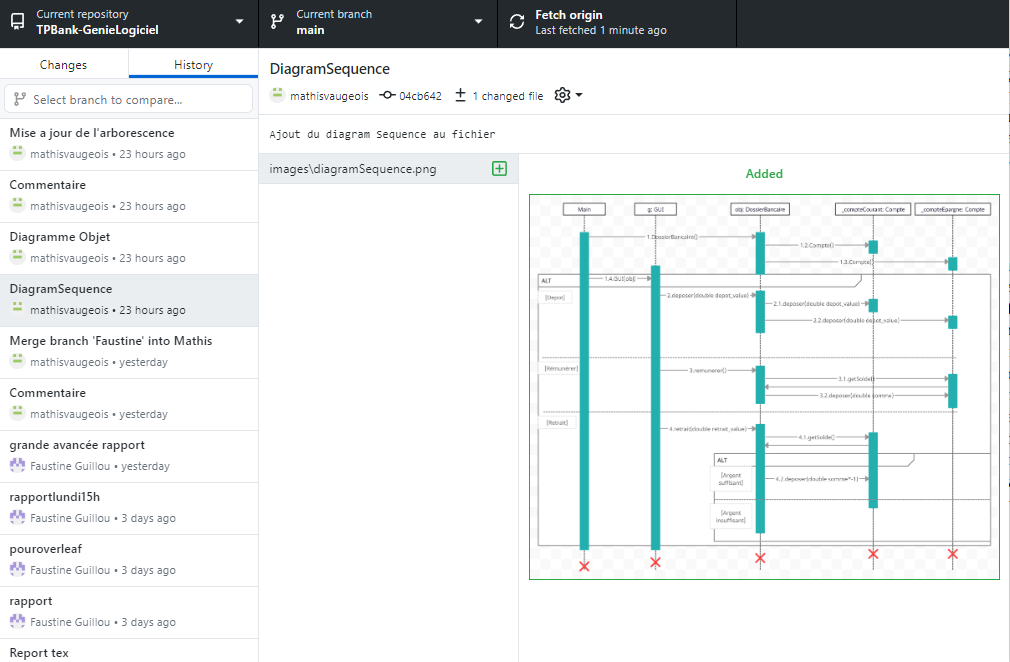
\includegraphics[width=0.8\textwidth]{interface githubdesktop}
\end{figure}
\newpage
Ci-dessus, on peut voir l'interface de github desktop, on peut notamment remarquer, en haut à gauche, le projet dans lequel on travaille (ici le projet du TP), un bouton juste a sa droite ou on peut choisir la branche (ici main) et un bouton avec plusieurs utiliser : il fetch pour vérifier la version en ligne sur github, pull si le projet en ligne et différent, et push si notre projet à des commit à publier (ici on est à jour et github aussi). La barre à gauche peut afficher deux onglets. Nous avons l'onglet Changes (ci-dessous) qui nous donne les changements en cours a commit (nous permettant de mettre un titre et une description) ainsi qu'un rendu des différences des fichiers modifier avec le précédent commits de la branche si l'application reconnaît le type du fichier (en général les images et les fichiers textes, dont les fichiers de code, sont reconnus). L'onglet History (ci-dessus) qu'en a lui, nous montre une liste défilante des commits avec la date de leur publication (ici elle est comparée à la date actuelle) et en sélectionnant un, on peut voir à droite le titre, la description ainsi que les différents fichiers qui ont été modifier et leurs changements tout comme l'onglet Changes (c’est-à-dire que le commit sélectionner est comparé avec le précédent).
\begin{figure}[h]
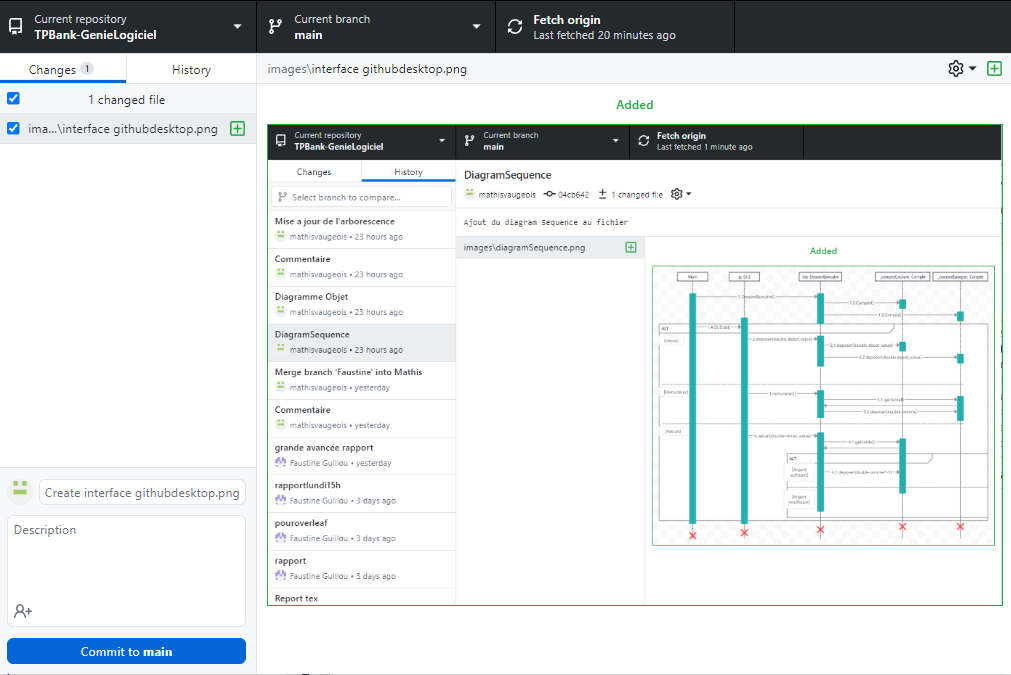
\includegraphics[width=0.8\textwidth]{Interface GithubDesktop 2}
\end{figure}

\newpage
\section{Cahier des charges}


\textcolor{Purple}{1. Proposez un diagramme UML de classes correspondant à ce cahier des charges.}
\newline
Pour réaliser le diagramme de Classe, nous avons d'abord travaillé sur feuille et nous l'avons mis au propee en utilisant InkScape. 
Nous avons décider de créer un seul type Compte, avec compte courant et compte épargne, deux entités différentes de Compte, car ils ont tous les deux les mêmes attributs.
Compte dépend entièrement de Dosier Bancaire, donc si le dossier bancaire est supprimé, les comptes le seront aussi.
\begin{figure}[h]
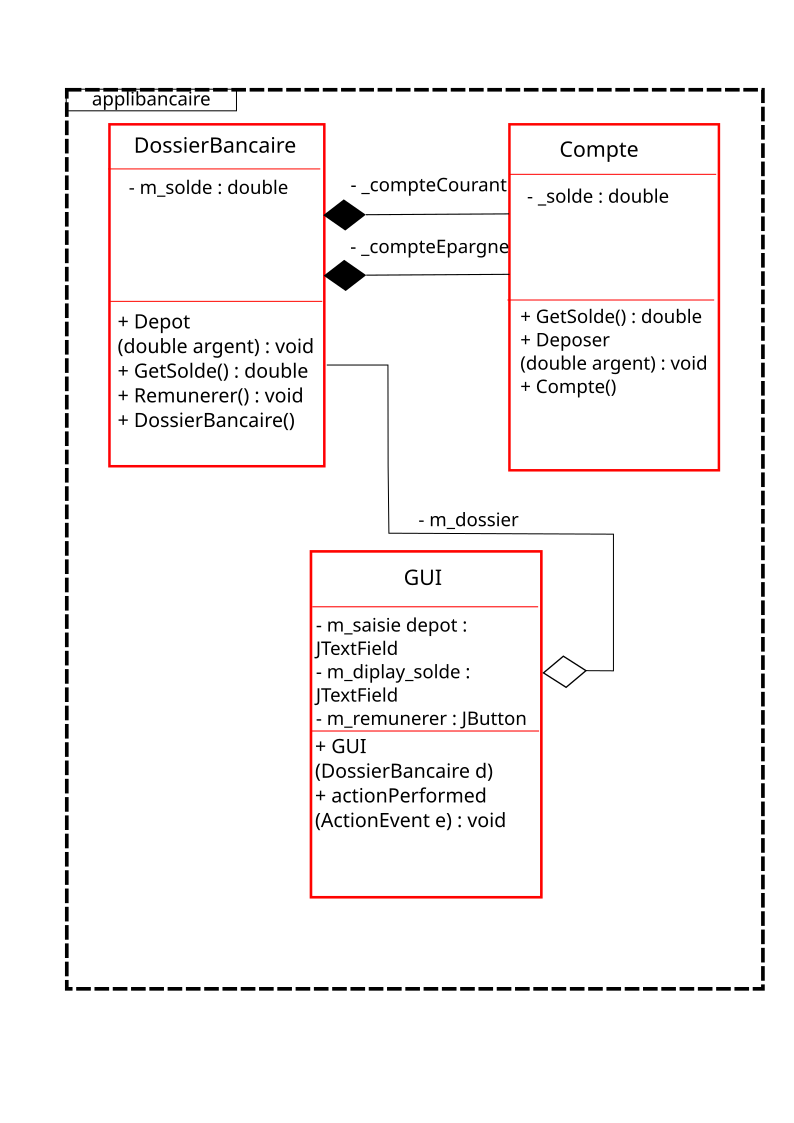
\includegraphics[width=0.8\textwidth]{diagrammeClasse.png}
\end{figure}
\newline
\newpage

\textcolor{Purple}{2. Donnez un diagramme UML de séquences illustrant les différents appels de méthodes et leurs relations.}
\newline
Nous avons ensuite réalisé un diagramme de Séquence. Il débute par le main, qui initialise DossierBancaire. Pour décider des actions, DossierBancaire dépend du GUI, c'est donc par ce dernier que se lance tous les ordres.
Le premier ordre est déposer(). Via le GUI, le dépot se lance, DossierBancaire dépose sur Compte Courant et Compte Epargne.
Pour rémunérer, on récupère d'abord le solde du compte avant de prélever.
Pour le retrait, il y a double situations. Si l'argent est suffisant, on retire, si il ne l'est pas, rien ne se passe.
Pour effectuer des retraits sur le compte, nous n'avons pas créé une fonction. Nous réutilisns déposer mais en utilisant un chiffre négatif dont la valeur absolue est égale à la valeur du retrait.
\begin{figure}[h]
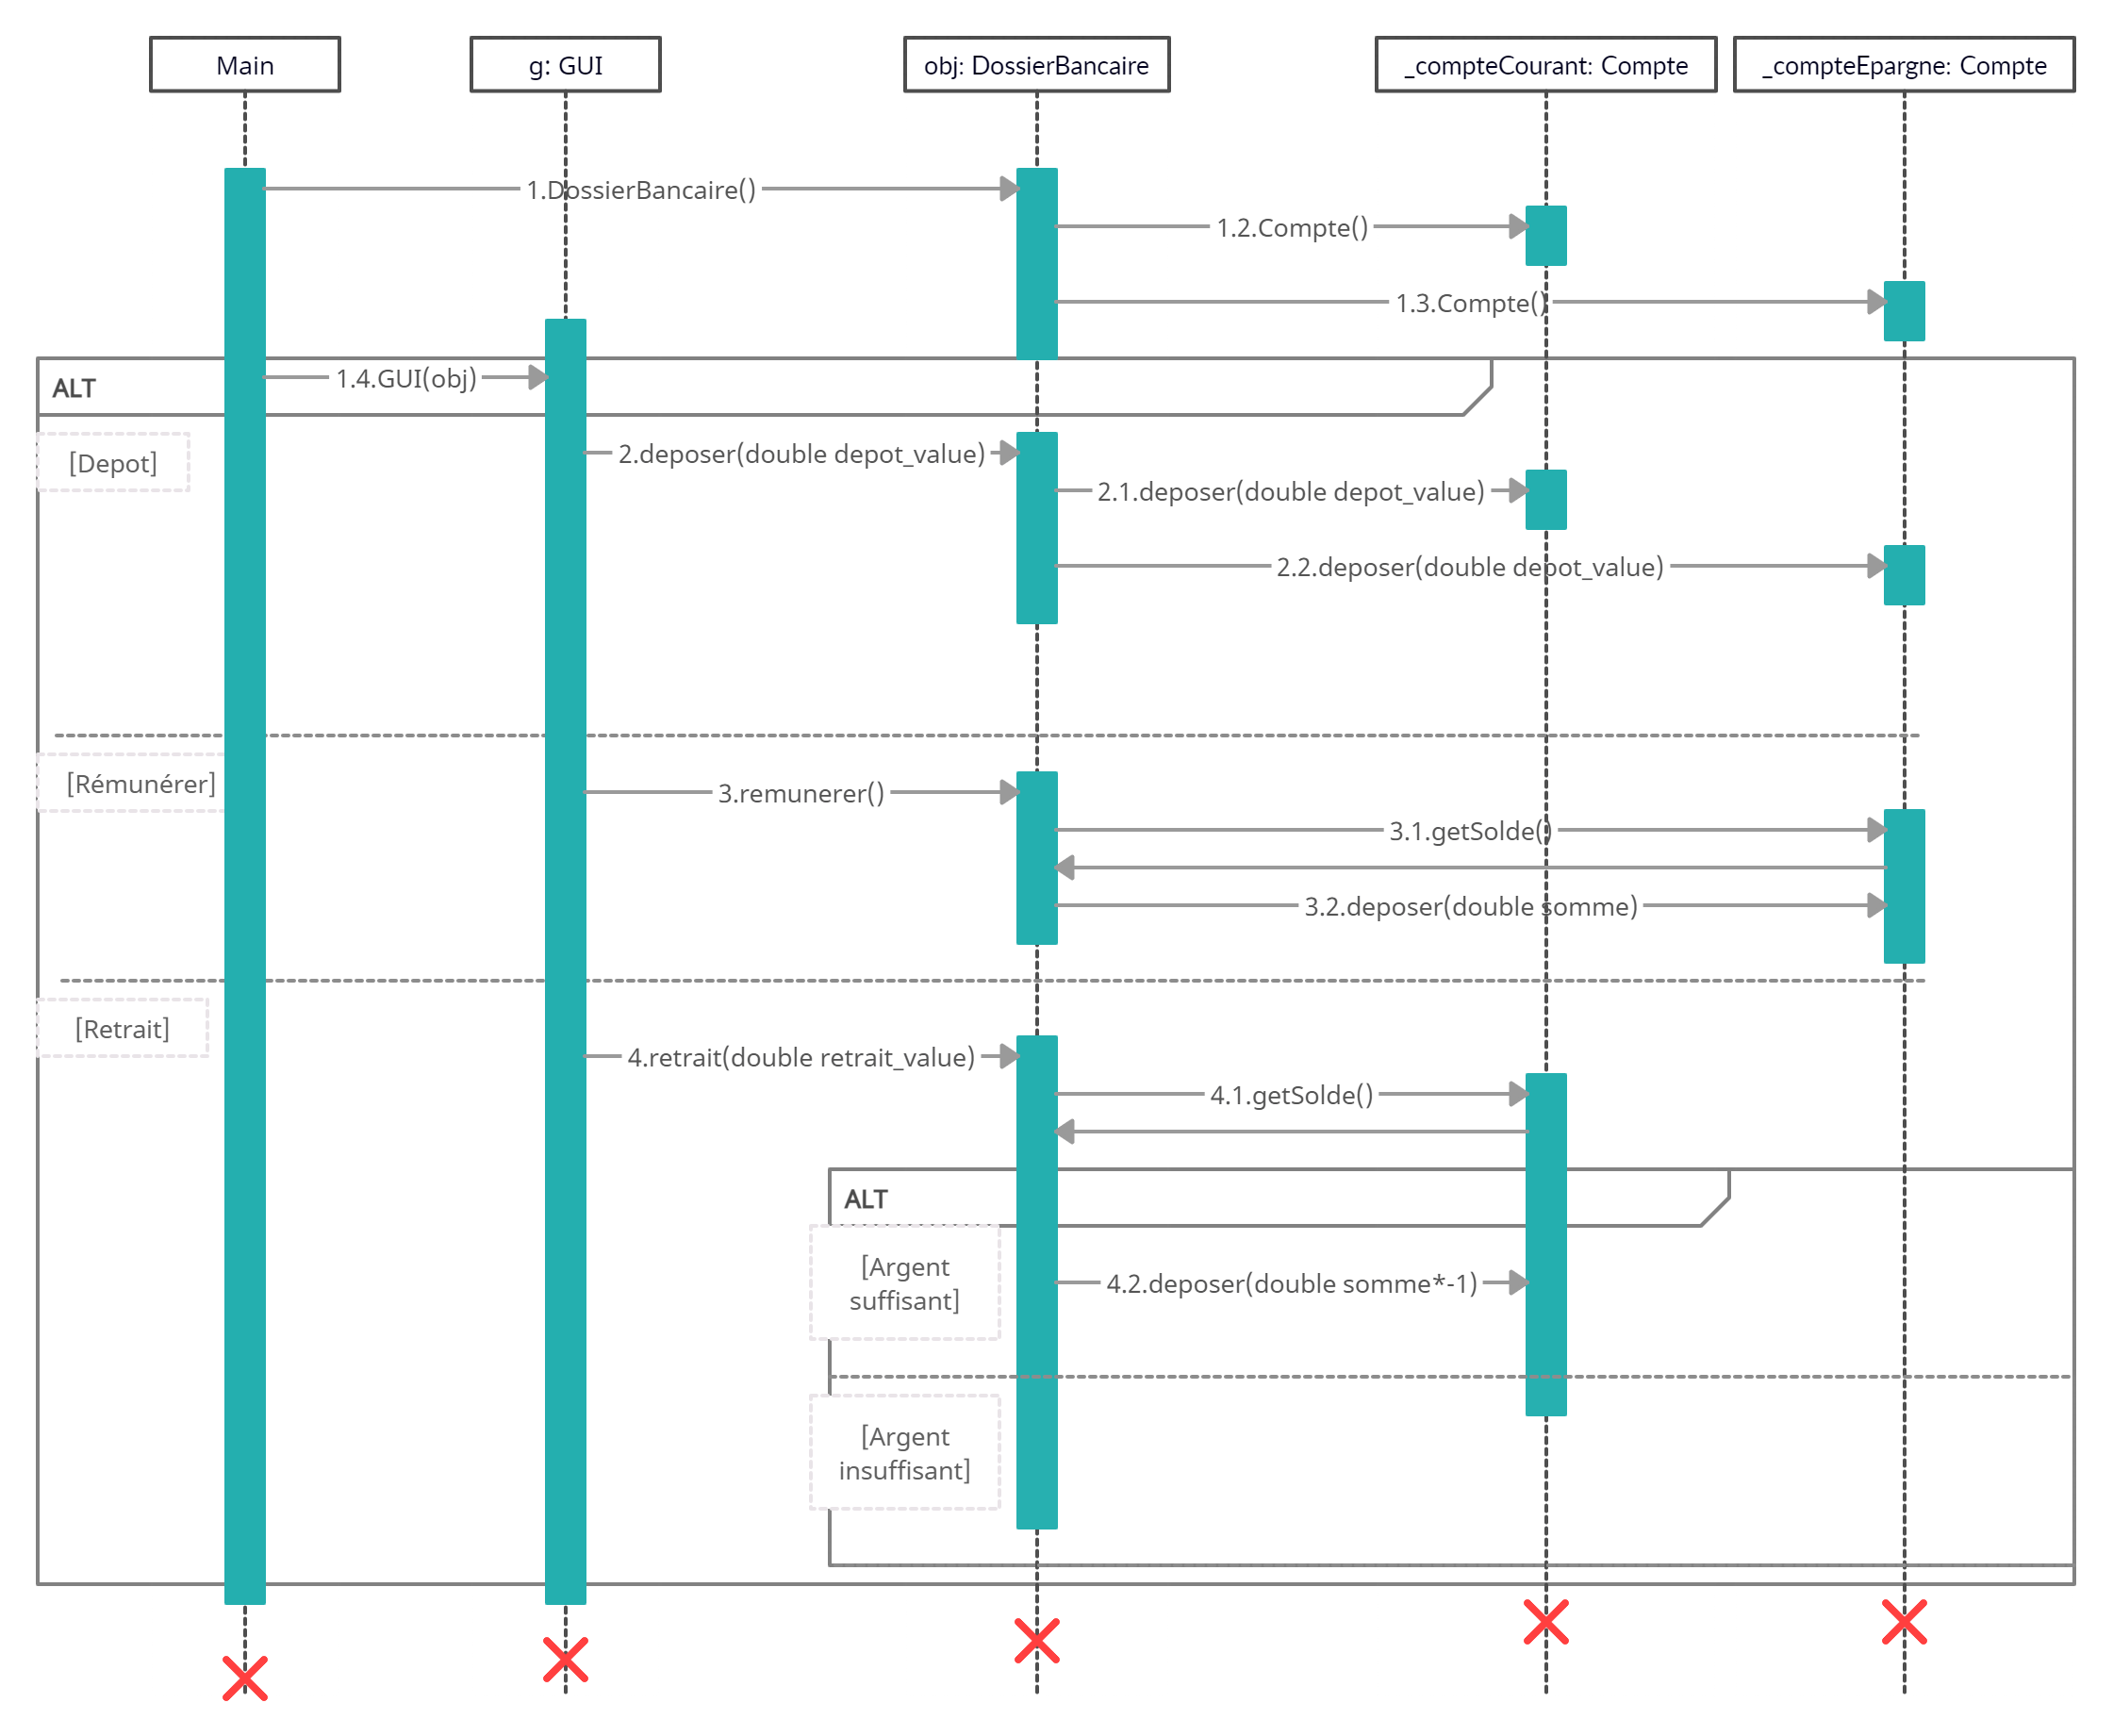
\includegraphics[width=0.8\textwidth]{diagramSequence-min.png}
\end{figure}

\textcolor{Purple}{3. Quel autre type de diagramme pourriez-vous proposer ?}
\newline
En plus des deux diagrammes précédents, nous pourrions aussi proposer un diagramme d'objets. Le voici donc:



\begin{figure}[h]
\includegraphics[width=0.8\textwidth]{diagrammeObj.png}
\end{figure}

Il permet de rapidement voir tous les objets intervenant dans cette situation: le main, le GUI, le dossier banaire et les deux types de compte.


\newpage
\section{Code de départ}


\textcolor{Purple}{3. Vérifier que vous parvenez, en ligne de commande, à compiler et exécuter le programme.)}
\newline



Après avoir ouvert le projet, nous avons récupéré les commandes données dans le README, cependant cela ne fonctionnait pas.
\newline

\begin{figure}[h]

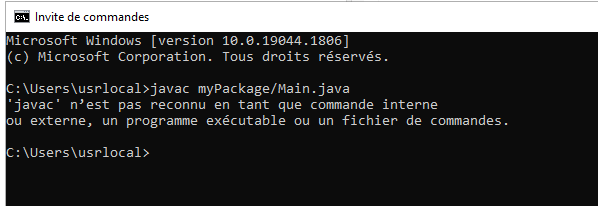
\includegraphics[width=1\textwidth]{erreurjavac.png}
\caption{Erreur de commande}
\end{figure}

 Le problème était que javac n'était pas reconnu en commande interne. Pour résoudre ce problème, nous avons ajouté javac au PATH.
 Nous avons ouvert la page Modifier les variables d'environnement dans le panneau de configuration.

\begin{figure}[h]

\includegraphics[width=0.8\textwidth]{Annotation 2023-01-10 143053.png}
\end{figure}

Ensuite, nous avons ouvert l'onglet variables d'environnement et avons modié le PATH de l'utilisateur usrlocal.

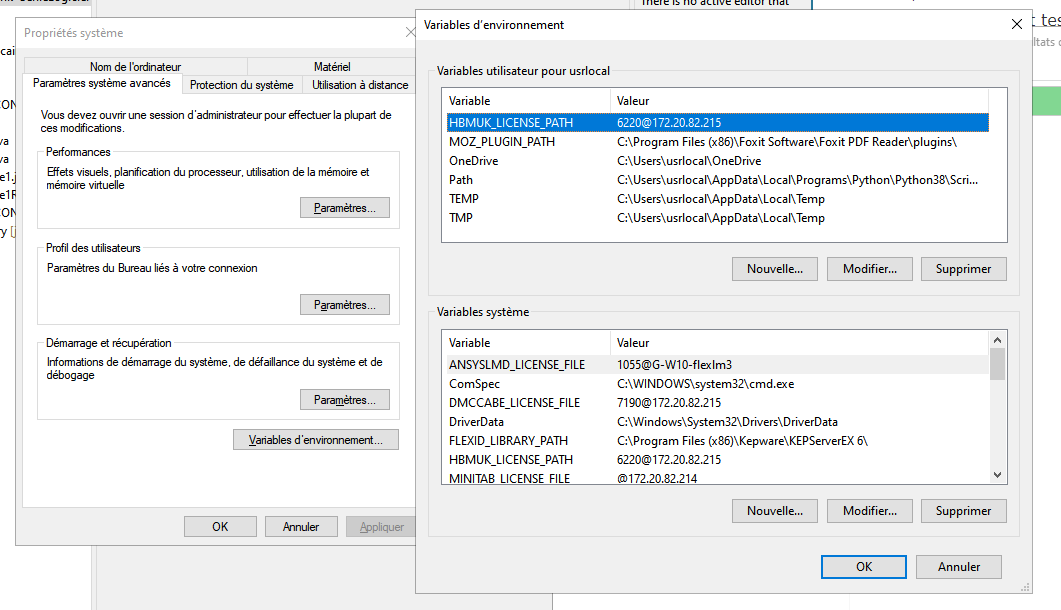
\includegraphics[width=0.8\textwidth]{Annotation 2023-01-10 143100.png}


Pour cela, nous avons du trouver le chemin de javac. Pour le trouver, nous avons tapé javac.exe dans l'explorateur de commande et avons trouvé que son chemin est C:/Program Files/Java/jdk-10.0.2/bin/javac.exe.
Nous avons ajouté le chemin du dossier dans lequel se trouve javac au PATH.


\begin{figure}[h]
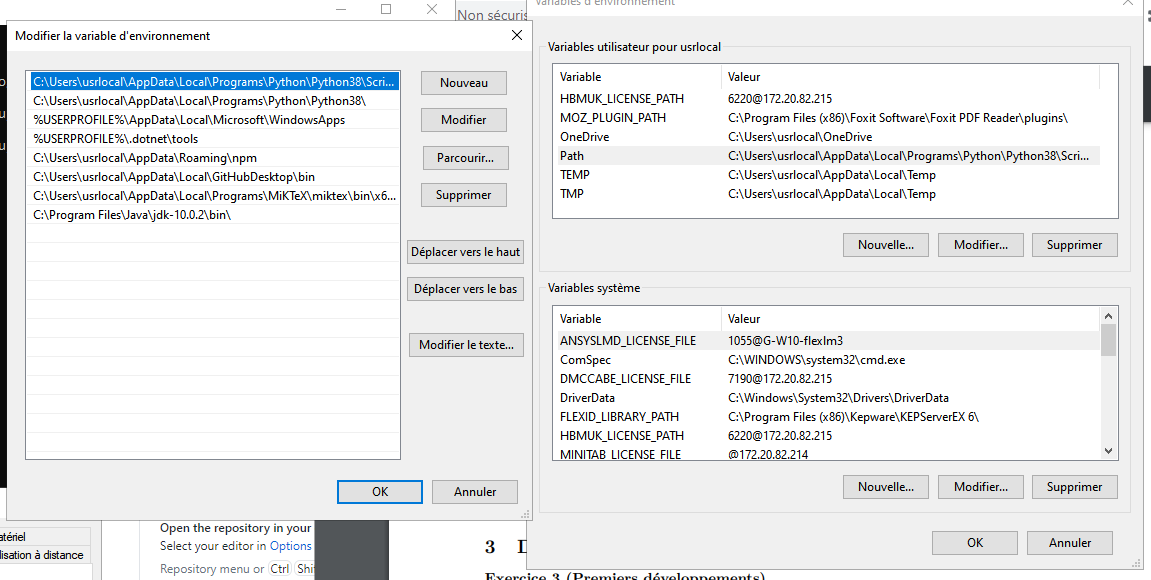
\includegraphics[width=0.8\textwidth]{Annotation 2023-01-10 145746.png}
\end{figure}
Ensuite nous avons pu relancer avec succès la commande compilation.
\begin{figure}[h]
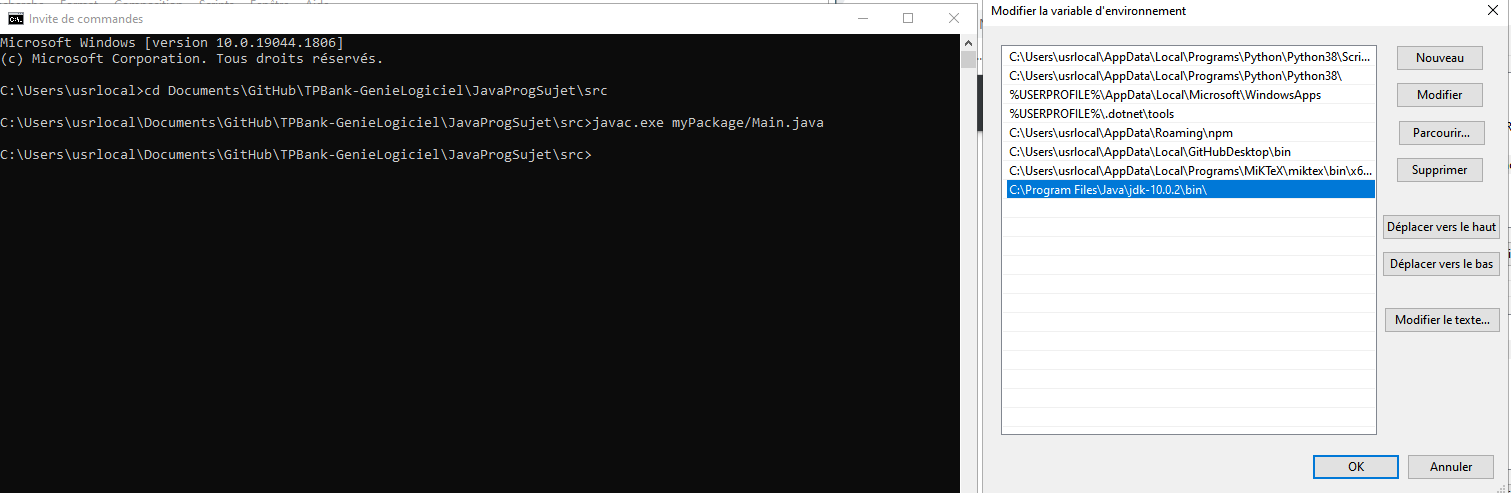
\includegraphics[width=0.8\textwidth]{Annotation 2023-01-10 145813.png}
\end{figure}

Si nous n'avions pas ajouté le chemin de javac aux path des variables d'utilisateurs, nous n'aurions pas pu utiliser la commande telle quelle. Il aurait fallu indiquer tout le chemin de javac.exe, ce qui est beaucoup plus long.
Après la compilation, le programme a pu s'éxécuter sans problème.

\newline
\textcolor{Purple}{4. Vérifiez que vous parvenez exécuter la suite de tests unitaires («Runner» fourni, intégrant
une méthode statique Main, déclenchant l’exécution de la suite de tests)}
\newline

La compilation et l'exécution des tests fonctionnent de manière similaire à celle du Main.
Nous avons tout d'abord récupéré la commande de compilation.

	
\begin{lstlisting}
javac -cp "C:\Program Files (x86)\eclipse\plugins
\org.junit_4.11.0.v201303080030\junit.jar";"C:\Program Files 
(x86)\eclipse\plugins\org.hamcrest.core_1.3.0.v201303031735.jar" 
tests\MyTest1.java tests\MyTest2.java ... etc...
\end{lstlisting}
Cette commande n'a pas fonctionnée.
Premièrement les chemins donnés étaient incorrects. De plus, il fallait ajouter tous les fichiers tests.
La commande est donc devenue :
\begin{lstlisting}
javac -cp "C:\eclipse\plugins\org.junit_4.13.2.v20211018-1956.jar";
"C:\eclipse\plugins\org.hamcrest.core_1.3.0.v20180420-1519.jar" 
tests\MyTest1.java tests\MyTest2.java tests\MyTestSuite1.java 
tests\MyTestSuite1Runner.java myPackage\DossierBancaire.java
\end{lstlisting}

Ensuite, nous avons exécuté les tests avec la commande :
\begin{lstlisting}
    C:\Users\usrlocal\Desktop\JavaProgSujet\src>java -cp 
    "C:\Program Files (x86)\eclipse\plugins\
    org.junit_4.11.0.v201303080030\junit.jar";
    "C:\Program Files (x86)\eclipse\plugins\
    org.hamcrest.core_1.3.0.v201303031735.jar"; tests/MyTestSuite1Runner
\end{lstlisting}

Comme la commande précédente, celle-ci n'a pas fonctionné. Les chemins étaient incorrects. La correction de la commande donne :

\begin{lstlisting}
    C:\Users\usrlocal\Desktop\JavaProgSujet\src>java -cp 
    "C:\eclipse\plugins\org.junit_4.13.2.v20211018-1956.jar"
    "C:\eclipse\plugins\org.hamcrest.core_1.3.0.v20180420-1519.jar"
    tests/MyTestSuite1Runner
\end{lstlisting}
\newpage
\section{Développement}

\subsection{Exercice 3 - Premiers développements}

\textcolor{Purple}{1. Créez un dépôt git (dans le répertoire du projet). Sous éclipse, bouton droit sur le projet,
«Team», «Share project», «git», sélectionner «use or create a repository in parent folder of project» puis «create repository», et finalement «finish». Le répertoire de votre projet éclipse doit contenir un sous-répertoire «.git/».}
\newline
\bigskip
Nous avions déjà créé le dépôt git au tout début, via GitHub.
\bigskip
\newline
\textcolor{Purple}{2. Ajoutez les fichiers (incluant les tests) de départ au dépôt git : «add to index» puis «commit».}

\newline
Comme pour la question précédente, cela était déjà fait.
\bigskip
\newline
\textcolor{Purple}{3. Ajustez les tests unitaires pour n’avoir qu’une seule classe de test «TestsDossierBancaire»
(on enlèvera les tests inutiles, et on (re)nommera correctement les fichiers). On implé-
mentera un test (méthode de la classe «TestsDossierBancaire») par méthode de la classe
DossierBancaire : il y aura ainsi 3 tests (incluant le constructeur). La «suite» sera donc
limitée à l’invocation des tests «TestsDossierBancaire» : on la renommera «TestsSuite».}
\newline
En premier lieu, nous avons retiré les tests inutiles. Nous avons déplacé les autres dans un fichier JUnit Test Case que nous avons nommé "TestDossierBancaire". De plus, nous avons écrit des tests supplémentaires pour tester les fonctionnalités de la classe DossierBancaire. Nous avons rajouté les tests 2,3 et 4. Nous avons ensuite renommé le fichier TestsSuites.
Voici le code du fichier de tests.

\begin{lstlisting}
   package tests;

import static org.junit.Assert.*;

import org.junit.Test;

import myPackage.DossierBancaire;

public class TestsSuite
{
	@Test  
	public void test1() 
	{
		DossierBancaire dossier = new DossierBancaire();
		dossier.deposer(100);
		assertEquals(100, dossier.get_solde(), 0);
	}
	
	
}
\end{lstlisting}
\textcolor{Purple}{4. Intégrez ces modifications à git et enfin «tagger» cette version initiale (V1.0)}
Nous avons intégrer ces modififications à git via GitHubDesktop. Nous avons d'abord commit et push les changements. Pour tagger cette version, nous avons fait un clic-droit sur la version en question dans l'history, et nous avons cliqué sur create tag.

\newline
\bigskip
\textcolor{Purple}{5. Ajoutez la classe compte courant seulement et intégrez la à la classe dossier bancaire : la
rémunération ne change pas le solde, et le dépôt sur le dossier bancaire est intégralement
affecté au compte courant. Ajouter les tests unitaires en conséquences et mettre la «suite»
à jour (l’exécution de celle-ci doit impliquer deux nouveaux tests : «constructeur» et «deposer»). Ajouter les deux fichiers à l’«index» et «Commiter» ces modifications.}
\newline
Une classe Compte a été créée. Celle-ci contient un solde (privé), ainsi qu'un constructeur et deux méthodes permettant de récupérer
le montant de ce solde, ainsi que de déposer de l'argent sur le compte.
\begin{lstlisting}
    package myPackage;

public class Compte
{
	private double solde;
	
	public Compte() 
	{
		solde = 0;
	}
	
	public double getSolde() 
	{
		return solde;
	}
	
	public void deposer(double somme) 
   
	{
		solde += somme;
	}
}
\end{lstlisting}
Un attribut de type Compte a été ajouté au dossier bancaire (compteCourant), permettant d'accéder aux comptes.
\begin{lstlisting}
    private double m_solde;
	private Compte _compteCourant;
	
	
    public DossierBancaire()
    {
    	m_solde=0;
    	Compte _compteCourant = new Compte();
    	
    }
\end{lstlisting}
La fonction déposer a été développée.
\begin{lstlisting}
    public void deposer(double argent)
    {
    	m_solde += argent;
    	_compteCourant.deposer(argent);
    }
\end{lstlisting}
Nous avons de plus rajouté une méthode avec d'accéder au compte couant.

\begin{lstlisting}
public Compte getCompteCourant()
    {
    	return _compteCourant;
    }
\end{lstlisting}


Ensuite, nous avons développé des tests pour ces changements.
\begin{lstlisting}

	
	@Test  
	public void test2() 
	{
		DossierBancaire dossier = new DossierBancaire();
		dossier.deposer(42);
		assertEquals(42, dossier.getCompteCourant().getSolde(), 0);		
	}
}
\end{lstlisting}

\newline
\bigskip

\textcolor{Purple}{6. Ajoutez la classe compte épargne («CompteEpargne») et intégrez la à la classe dossier bancaire : la rémunération change le solde, et le dépôt sur le dossier bancaire est ventilé entre les deux comptes. Ajouter les tests unitaires sur «CompteEpargne», ajustez ceux sur «DossierBancaire» et «Commiter» ces modifications.}
\newline
Un attribut de type Compte a été ajouté au dossier bancaire (compteEpargne), permettant d'accéder aux comptes.
\begin{lstlisting}
    private double m_solde;
	private Compte _compteCourant;
	private Compte _compteEpargne;
	
    public DossierBancaire()
    {
    	m_solde=0;
    	Compte _compteCourant = new Compte();
    	Compte _compteEpargne = new Compte();
    }
\end{lstlisting}
La fonction déposer a été modifiée, pour inclure le compte épargne.
\begin{lstlisting}
     public void deposer(double somme)
    {
    	m_solde += somme;
    	_compteCourant.deposer(0.4 * somme);
    	_compteEpargne.deposer(0.6 * somme);
    }
\end{lstlisting}
Le dossier bancaire contient aussi désormais une fonction de rémunération à taux fixe, qui dépose de l'argent sur le compteEpargne.
\begin{lstlisting}
    public void remunerer()
    {
    	double somme = _compteEpargne.getSolde();
    	somme = 0.032 * somme;
    	_compteEpargne.deposer(somme);
    }
}
\end{lstlisting}
Nous avons aussi ajouté une méthode pour accéder au compte épargne.
\begin{lstlisting}
public Compte getCompteEpargne()
    {
    	return _compteEpargne;
    }
    
\end{lstlisting}

Ensuite, nous avons développé des tests pour ces changements.
\begin{lstlisting}
@Test  
	public void test3() 
	{
	   DossierBancaire dossier = new DossierBancaire();
	   dossier.deposer(100);
      assertEquals(60, dossier.getCompteEpargne().getSolde(), 0);	
	   dossier.remunerer();
	   assertEquals(61.92, dossier.getCompteEpargne().getSolde(), 0);	
	}
\end{lstlisting}

Nous avons intégré ces modifications via GitHub Desktop en commitant.
\bigskip

\bigskip

\textcolor{Purple}{7. Taggez cette version en 2.0.}
\newline
Pour tagger cette version, nous avons fait un clic-droit sur la ersion en question dans l'history, et nous avons cliqué sur create tag.

\bigskip

\textcolor{Purple}{8. Testez le retour la version antérieure 1.0 (sélection du tagV1.0 dans «team History», bouton droit et «checkout») : consulter les fichiers, exécutez l’application (avec IHM : la rémuneration est inactive), les tests unitaires.}
\newline
Pour revenir à la version souhaitée, nous avons utilisé GitHub Desktop. Nous nous sommes placés sur le branche correct (main) et dans history, nous avons sélectionné le commit souhaité. Nous avons ensuite executé et testé la version en question.

\bigskip

\textcolor{Purple}{9. Revenez finalement à la dernière version (V2.0).}
\newline
Nous avons utilisé le même processus pour revenir à la dernière version.

\bigskip


A la fin de l'exercice, nous avons pu admirer ce graphique :

\begin{figure}[h]
\includegraphics[width=0.8\textwidth]{historyexo3.png}
\end{figure}

\subsection{Exercice 4 - Fusion}

\bigskip

\textcolor{Purple}{1. Modifiez la classe DossierBancaire (e.g. documentation, renommage attribut) puis commiter.}
\newline
Afin de répondre à cette question, nous avons légèrement modifié la classe DossierBancaire en ajoutant des commentaires.
\begin{lstlisting}
     package myPackage;

public class DossierBancaire
{	
	private double m_solde;
	private Compte _compteCourant;
	private Compte _compteEpargne;
	
    public DossierBancaire() //constructeur du dossier bancaire
    {
    	m_solde=0;
    	_compteCourant = new Compte();
    	_compteEpargne = new Compte();
    }

    public void deposer(double somme) //déposer de l'argent sur les deux comptes courant et épargne
    {
    	m_solde += somme;
    	_compteCourant.deposer(0.4 * somme);
    	_compteEpargne.deposer(0.6 * somme);
    }
    
    public double get_solde() //renvoie le solde du dossier
    {
    	return m_solde = _compteCourant.getSolde() + _compteEpargne.getSolde();
    }
    
    public Compte getCompteCourant() //renvoie le compte courant
    {
    	return _compteCourant;
    }
    
    public Compte getCompteEpargne() //renvoie le compte épargne
    {
    	return _compteEpargne;
    }
    
    public void remunerer() //verser les intérêts sur le compte épargne
    {
    	double somme = _compteEpargne.getSolde();
    	somme = 0.032 * somme;
    	_compteEpargne.deposer(somme);
    }
}
\end{lstlisting}
\begin{figure}[h]
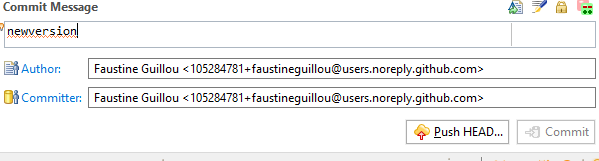
\includegraphics[width=0.8\textwidth]{commit.png}
\end{figure}
\bigskip

\textcolor{Purple}{2. Revenez à la version «2.0», créez une branche nommée newdev et modifiez, sur cette branche, le code : amélioration de la structure du code en intégrant l’héritage afin de
factoriser des éléments des classes compte courant et compte d’épargne (faites au moins deux étapes -i.e. deux commits pour enrichir la branche).}
\newline

Faisable avec GitDekstop. Amélioration de la structure du code précédemment réalisée (lors de l'initialisation du projet). Documentation enrichie.

\bigskip

\textcolor{Purple}{3. Revenez sur la branche principale («master») et faites de nouvelles modifications mineures sur la classe Dossier Bancaire (sans créer de conflit : par exemple ajoutez des
commentaires).}
\newline 
Nous avons intégrés des commentaires afin d'effectuer des modifications.
\begin{lstlisting}
    public class DossierBancaire
{	
	private double m_solde; //solde général des deux comptes bancaires
	private Compte _compteCourant; //Element de la classe Compte
	private Compte _compteEpargne; //Si on en veut plusieurs on peut facilement passé sa en liste et modifier les fonctions
	
    public DossierBancaire() //constructeur du dossier bancaire
    {
    	m_solde = 0;
    	_compteCourant = new Compte(); //Creation d'un compte
    	_compteEpargne = new Compte();
    }

    public void deposer(double somme) //déposer de l'argent sur les deux comptes courant et épargne
    {
    	m_solde += somme;
    	_compteCourant.deposer(0.4 * somme); //Depose 40% de la somme
    	_compteEpargne.deposer(0.6 * somme); //Depose 60% de la somme
    }
    
    public double get_solde() //renvoie le solde du dossier
    {
    	return m_solde = _compteCourant.getSolde() + _compteEpargne.getSolde();
    }
    
    public Compte getCompteCourant() //renvoie le compte courant
    {
    	return _compteCourant;
    }
    
    public Compte getCompteEpargne() //renvoie le compte �pargne
    {
    	return _compteEpargne;
    }
    
    public void remunerer() //verser les intérêts sur le compte épargne
    {
    	double somme = _compteEpargne.getSolde(); //Recupere le solde actuelle
    	somme = 0.032 * somme; //Fait le calcul
    	_compteEpargne.deposer(somme); //Mise a jour le solde
    }
    
    public void retrait(double somme)
    {
    	double current_value = _compteCourant.getSolde(); //Recupere le solde
    	if(somme <= current_value)
    	{
    		//OK POUR LE RETRAIT
    		_compteCourant.deposer(-somme);    		
    	}
    	else
    	{
    		//PAS OK POUR LE RETRAIT
    		//SEND ERREUR
    		System.out.println("Solde insuffisant");
    	}
    }
}
\end{lstlisting}

\bigskip

\textcolor{Purple}{4. Intégrez les modifications de la branche «newdev», en revenant au préalable sur le «master».}
\newline

Sur GitHub Desktop, nous sommes revenus sur la branche master, puis nous avons sélectionné une branche à intégrer dans main, ici newdev.




\begin{figure}[!h]
\includegraphics[width=0.8\textwidth]{merge.png}
\end{figure}


\bigskip
\newpage
\bigskip

\textcolor{Purple}{5. Vérifiez le bon fonctionnement de l’application.}
\newline
Après vérification, les tests et le GUI fonctionnent parfaitement.

\begin{figure}[!h]
\includegraphics[width=0.8\textwidth]{gui.png}
\end{figure}
\newpage
A la fin de l'exercice, nous avons pu admirer ce graphique :

\begin{figure}[h]
\includegraphics[width=0.8\textwidth]{historyexo4.png}
\end{figure}
\newpage
\newpage
\subsection{Exercice 5 - Tests}
\bigskip

\textcolor{Purple}{1. Ajoutez la possibilité de retirer de l’argent du dossier bancaire : on considérera qu’un tel retrait n’altère que la classe Compte Courant, et qu’une exception est levée si le solde
est insuffisant.}
\newline
Une fonction de retrait a été ajoutée à la classe DossierBancaire et permet de retirer de l'argent du compteCourant, avec vérification du solde préalable à l'opération.

\bigskip

\textcolor{Purple}{2. Faites en sorte que la levée de cette exception soit vérifiée par le test unitaire associée
(voir documentation JUnit).}
\newline
Nous avons mis en place un test JUnit pour vérifier que la fonction de retrait fonctionne correctement.
\begin{lstlisting}
    @Test  
	public void test4()
	{
		DossierBancaire dossier = new DossierBancaire();
		dossier.deposer(100);
		dossier.retrait(30);
		assertEquals(10, dossier.getCompteCourant().getSolde(), 0);
	}
\end{lstlisting}

\bigskip

\textcolor{Purple}{3. Modifiez la classe «GUI», pour permettre un retrait depuis l’interface graphique.}
\newline
Ensuite, nous avons modifié l'interface GUI, afin de permettre d'intégrer la fonctionnalité de retrait.

\begin{lstlisting}
    public class GUI implements ActionListener 
{
	private DossierBancaire m_dossier;
	private JTextField m_saisie_depot;
	private JTextField m_display_solde;
	private JButton m_remunerer;
	private JTextField m_saisie_retrait;

 //ajout du JTextField m_saisie_retrait
	
\end{lstlisting}
\begin{lstlisting}
     //Element saisie retrait
        m_saisie_retrait = new JTextField (20);
        m_saisie_retrait.addActionListener(this);


       frame.getContentPane().add(m_remunerer); 
        frame.getContentPane().add(new JLabel("Retrait"));
        frame.getContentPane().add(m_saisie_retrait);

        if( e.getSource() == m_saisie_retrait )
    	{
    		double retrait_value=Double.parseDouble
            (m_saisie_retrait.getText());
    		m_dossier.retrait(retrait_value);
    		m_saisie_retrait.setText("");
    	}
    	m_display_solde.setText(Double.toString(m_dossier.get_solde())); 
\end{lstlisting}

\bigskip

\textcolor{Purple}{4. Pensez avec «versionner» cette nouvelle version «3.0».}
\newline
Après avoir fait ces nouvelles modifications, nous avons commit sur GitHub Desktop. Ensuite, nous avons push. Dans l'interface history énumérant tous les commit, nous avons fait un clic droit sur le dernier et avons sélectionné create tag.

Tout au long de la partie concernant Eclipse, nous avons alterné entre Eclipse et GitHub Desktop pour commit nos changements. Les deux fonctionnent tout aussi bien l'un que l'autre. La seule différence entre les deux interfaces sont les fichiers commit. Eclipse ne commit que le projet lui-même. Avec Github, nous pouvons commit en même temps d'autres fichiers faisant parti du dépôt mais étant en dehors du projet Eclipse. C'est cette difféence qui a déterminé l'alternance entre ces deux interfaces.
\section*{Référence}
\url{https://github.com/mathisvaugeois/TPBank-GenieLogiciel}

\end{document}